\chapter{Syntax, Labels, and Jazz}

\section{Jazz Harmony and Syntax}
%Mehegan's call to figured bass
In the first volume of his incredibly thorough pedagogical series \emph{Jazz Improvisation}, John Mehegan makes a series of bold claims regarding jazz harmony.  Here is a summary of two of these claims, from which and against which I hope to stake out my goals and methods in the study of jazz harmony:
\begin{enumerate}
	\item Jazz harmony ``is classical harmony following the identical rules and conventions found in a Bach fugue, a Mozart sonata, a Brahms rhapsody."\footnote{Mehegan 1959, p.\ 7.}
	\item ``The use of chord letters among musicians may seem strange when one considers that an organized method of spelling any musical function has existed for some two hundred years-- Figured Bass... In other words, the jazz musician plays by the natural system of figured bass."\footnote{Ibid., p.\ 8.}
\end{enumerate}
Mehegan's project is to describe the jazz piano repertoire in a manner systematic enough to allow pianists to replicate the stylistic harmonies, voicings, rhythms, and melodic lines of prominent performers.  This teaching machine hums along quite well, if the praise of performers and theorists who have worked with it is taken as its output.\footnote{The series is explicitly endorsed in prefaces and introductions by Leonard Bernstein (Vol.\ 1), Horace Silver (Vol.\ 3), and Bill Evans (Vol.\ 4), among others.}  The two claims above give us a glimpse under the hood of the machine, and I consider them emblematic of two recurring themes in jazz harmonic studies.  Claim (2) is primarily one of chord labeling, and I will return to it in \S 2 and 3 below.  Claim (1), regarding the ``rules and conventions" of jazz and classical music, seems to me to indicate something about the allowable patterns of harmonic progression in both genres.  The chords literally deployed in ``classical harmony" and jazz are not usually expected to be the same,\footnote{For example, the primarily triadic surfaces of western common practice tonality seem to differ from the extended voicings frequently found in jazz performances.} so Mehegan's claim seems to mean that the rules and conventions are an abstraction from the musical surface, in both cases.  Tonal theories which abstract away from the surface particulars in some way in order to reveal harmonic rules and conventions have often been described as theories of \emph{syntax} since the early 1960s.\footnote{Following the publication of Chomsky 1957 and 1965, music theory works like Winograd 1968, Lerdahl and Jackendoff 1977, and Steedman 1984 draw on syntactic terms and methods.  See \S 4 for an overview of this line of thought.}

My aim here is to produce a robust and flexible ground for investigating jazz syntax.  Theories which address stylistic chord progressions in jazz already exist; some of them explicitly invoke syntax, while others do not.  To contextualize my own pursuit of jazz syntax, I will briefly summarize extant harmonic approaches ranging from the purely pedagogical to the abstractly theoretical.  The limitations of and assumptions behind these theories will then motivate the project which follows.

\subsection{Pedagogical Approaches}
%Mehegan (though not really), Coker, Levine, Russell
Pedagogical approaches to jazz harmony usually aim to turn non-jazz musicians into jazz musicians, assuming the abilities to read music notation and handle instrumental technique and instructing the player as to what chords and melodies he or she may use to play in various jazz styles.  Mehegan's manual does this primarily via transcription.  He explains a chord labeling technique (his ``figured bass," which will occupy the majority of \S 3 below) and provides instructions for how to realize his labeled chords on the piano.  With these instructions on the table, he can provide self-composed practice exercises and transcriptions of famous tunes, teaching primarily by example instead of through the explication of syntactic theories.\footnote{Mehegan appeals to chord function and circle-of-fifths progressions to justify his chord labeling techniques, and these statements might reveal a latent theory of syntax lurking behind his examples.  For now, it suffices to say that Mehegan's chord labeling work is closely linked to functional and syntactic concerns but spends little time explicating them.  (See \S 3.)}

%Coker
Works like Coker's \emph{Improvising Jazz} (1964) provide a chord labeling system plus a harmonic theory meant to summarize which kinds of progressions show up in jazz and distill them down to a few rules.  Learning only the ``chord symbols and chord structures found in jazz," Coker claims, would be like ``learning the alphabet and vocabulary of a foreign language and, without knowledge of the syntax or structure, attempting to speak the language."\footnote{Coker 1964, p.\ 71.}  This quasi-linguistic syntax and structure is captured by Coker's categories of chord function, each of which is indexed by a collection of relevant roman numerals (RNs).  The simplest form of this functional syntax can be based entirely on chords labeled V$^{7}$, II$^{m7}$, and I$^{M7}$, which ``comprise approximately 75 per cent of all chords."\footnote{Ibid., p.\ 75.}  These chords progress along the circle of fifths such that each chord's root descends by a fifth to the next appropriate chord: hence, the all-pervasive II-V-I progression in jazz.

If we label the chords we find in a jazz tune as stacks of thirds with roots indicated by RN, Coker explains that we will find patterns of chord configurations (that is, their pitch structures) and chord successions (that is, the progressions from harmony to harmony).  The tonic family consists of major seventh chords and ``minor tonics" (consisting primarily of minor triads with an added sixth and major-minor seventh chords); these chords carry connotations of stability.  ``The minor sevenths," as a class of chord configurations, ``function as \emph{subdominants}," in that they are ``remote from the tonic and act as a secondary tonic."\footnote{Ibid., p.\ 71.}  Dominant sevenths lean strongly toward tonics, rounding out the functional categories necessary to account for harmonic phrases.  This identification of chord configuration with function (where function seems to mean ``role in a harmonic progression," determined largely by what chords progress to and from a given harmony) helps Coker to interpret strings of chord symbols as RNs.  If minor sevenths usually function as subdominants, and II is the most common subdominant, we should guess that the appropriate label for Am7 is II$^{m7}$, context permitting.\footnote{I note here, in passing, that Coker invokes intuitions about syntax in order to help him make labeling decisions; to use the resulting patterns of labels as proof of the syntax would be circular.  This is not a unique occurrence in jazz chord labeling practices, and I will return to it at length in Chapter 5.}  With these instructions in mind, let us try to identify the functional syntax of a very brief example, given in Figure~\ref{levine_folks}.
%FIGURE 1: Levine Figure 3-1, p. 17
\begin{figure}
	\centering
	\caption{The first two bars of Hill-Robinson's ``Old Folks," as annotated and included in Levine 1989, p.\ 17.}
	\label{levine_folks}
	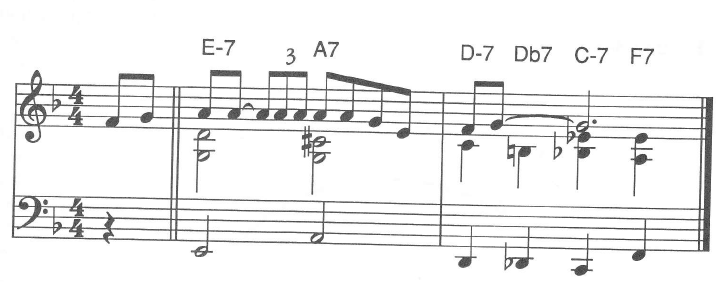
\includegraphics[width=5in]{levine_31.png}
\end{figure}

We first notice that most of the chords, as indicated by the associated chord labels, are incomplete; while the A7 chord contains root, third, fifth, and seventh, most of the other chords lack a fifth, and the ``D$\flat$7" chord also lacks a third.  If we are to apply Coker-style RNs, we will have to treat them as categories where entities like $(EGD)$ and $(EGBD)$ can both be called some kind of minor seventh chord.\footnote{Coker devotes little prose to voicing and omitted notes, but he does include a helpful Appendix B of suggested voicings; see pp.\ 83-84.}  The implied structures of the first two chords would then lead us to label them as II$^{m7}$ and V$^7$ in the key of DM.  The dominant chord should bring back the tonic chord, but what follows is a minor seventh chord (D-7) instead of a major or major-minor seventh.  For Coker, are these three chords a functional II-V-I progression?  The second bar contains two more minor seventh to dominant seventh progressions, the first of which does not reflect root motion on the circle of fifths.  Coker ultimately accounts for progressions like D$^{m7}$-D$\flat^7$-C$^{(M)7}$ by placing chords like $\flat$II$^7$ into the ``dominant" category on the basis of their intervallic structure and use, rather than their root motion.\footnote{See the table of equivalent functions given on p.\ 80.}  He does not, however, tell us whether we should call the D-7 in our example a tonic minor seventh (I$^{m7}$ in D), a subdominant minor seventh (II$^{m7}$ in C), or both.

%Levine
The example itself, the first two bars of Hill-Robinson's ``Old Folks," is annotated by Mark Levine and included in \emph{The Jazz Piano Book} (1989).  Like Coker 1964, Levine 1989 is a pedagogical treatise for the aspiring jazz player.  But instead of focusing on functional families of RNs, Levine identifies chords and progressions based solely on their most frequent usages.  This occasionally aligns him with Coker's subdominant-dominant-tonic (SDT) paradigm (as in his Chapter 2), but on other occasions it leads Levine to identify principles dictating chord progressions based on voicing or voice-leading concerns.  His Figure 3-1, reproduced as my Figure~\ref{levine_folks} above, is given an explanation of this type: while we might find II-V-I progressions in the passage, the more important observations, to Levine, are the root descents by fifth (except for the tritone substitution D$\flat^7$) and the consistent voice-leading pattern whereby the seventh of each chord descends by step to the third of the chord that follows.  The remainder of his work provides case studies of many chords and voicings which fall outside standard tertian labels and SDT harmony, and his approach is notable for its pluralism.\footnote{These case studies lead Levine to speculate about the best ways to label and explain such sonorities, and the results are sometimes thorny.  See \S 3 below for an illustrative example.}  While Levine's bag-of-tools approach provides helpful windows into particular forms of jazz harmonic practice, it does not provide a generalizable method for understanding the rules and conventions in play in many circumstances outside of his case studies, and it does not attempt to replace SDT syntax with any other conceptual framework.

Coker's conceptual simplicity and Levine's descriptive pluralism both fail to help us in the case of Figure~\ref{monk}, the opening 8 bars of Thelonious Monk's solo performance ``Memories of You."  For Coker to interpret RN functional progressions from the chord symbols supplied by the transcriber, he would first need to account for cases where the chord symbols themselves are wrong or misleading.  In m.\ 6, where is the $\flat$5 of the ``D$\flat 9\flat 5$" chord?  And what differentiates it from an inverted E$\flat^{7\flat 5}$ chord?  Even if the chord symbols all accurately represented Monk's musical surface, the unusual chord voicings and pitch structures would prevent us from assigning clear RNs or SDT functional labels.  Levine's attention to voicings might help us to identify a few more likely chord structures.  His observation in chapters 7 and 8 that dominant chords often replace a 5th with a 13th and employ a $\flat$9th might help us to contextualize the E13$\flat$9 of m.\ 5 as an altered dominant of the following Am chord;\footnote{See Levine 1989, pp.\ 41-58.} this functional association is strengthened by the circle-of-fifths root motion.  If one wanted to continue that reading, the ``D$\flat$9$\flat$5 C9" of m.\ 6 might be contested in favor of D9 (with no 3rd) preceded by a chromatic embellishing chord (E$\flat$7$\flat$5/D$\flat$). That would produce a descending 5ths sequence in mm.\ 5-8, starting on B and ending on F$^{M9}$ (the global tonic) in m.\ 9.   But such a reading does not demonstrate the necessity of a particular syntactic principle.  Rather, it \emph{assumes} syntactic principles and attempts to reduce the surface to those assumptions.
%FIGURE 2: Monk's ``Memories of You," the weird chord in m. 5
\begin{figure}
	\centering
	\caption{The opening 8 bars of Thelonious Monk's solo performance ``Memories of You."  Transcription taken from \emph{Thelonious Monk plays standards}.}
	\label{monk}
	\includegraphics[width=6in]{diss_prospectus_monk.png}
\end{figure}

%Russell
Pedagogical manuals like Mehegan's, Coker's, and Levine's are only indirectly meant for analytical tasks, and their descriptions of harmonic progressions in jazz can train jazz musicians without providing a method for investigating cases like Monk's above.  Some pedagogical works even seem to directly contradict the inclinations of analysts while aiding the performer: George Russell's \emph{Lydian Concept of Tonal Organization} (1953) employs an infamously idiosyncratic RN notational system to lay out the basis for his highly influential chord-scale theory.  Russell provides instructions for determing the ``parent scale" of every chord.  This parent scale will allow the improviser to construct melodic lines which sound appropriate over the harmony under consideration.  Russell determines the parent scale for a chord by seeing which scales can accomodate the notes of the chord most readily.  He then assigns the chord a RN based on its intervallic distance from the ``lydian tonic" of that scale.

The melodic possibilities for improvisers are rich, but the implications for RN syntax are dire.  Both chords of an E$\flat ^7$-A$\flat^{M7}$ progression, for example, draw notes from the D$\flat$ Lydian parent scale.\footnote{For Russell's description of E$\flat^7$ and the D$\flat$ Lydian scale, see pp.\ 4-15.  Note that my hypothetical A$\flat^{M7}$ could also be based on the tonic of the A$\flat$ Lydian scale; Russell will later appeal to this fact and calculate chord-to-chord distances based the distance between the parent scales of chords, rather than the distance between the chords within a single Lydian parent scale.}  Based on the distances of the chord roots above the Lydian tonic (D$\flat$), Russell might initially seem to suggest RNs II$^{(7)}$ and V$^{(M7)}$ (in D$\flat$ Lydian) where most analysts would indicate V$^{(7)}$-I$^{(M7)}$ (in A$\flat$ Major).  Since A$\flat$ Major and D$\flat$ Lydian share the same diatonic collection, this amounts to a change of centricity, and the RNs correspondingly don't seem to align with their traditional uses.

To partially mitigate this, Russell postulates a separate ``over-all parent Lydian Chromatic Scale," in which he tracks chord-to-chord motions within a piece; the key of the piece is meant to correspond to the Lydian tonic of the over-all parent Lydian Chromatic Scale.\footnote{The Lydian Chromatic Scale is simply a somewhat-misleadingly named chromatic scale.  It receives its unusual moniker by subsuming the (variously altered) Lydian scales which share its Lydian tonic.  See Lesson II, pp.\ 9-15.}  Chord progressions are then captured in Russell's system by attending to the distances between the parent scales of each chord relative to the over-all parent Lydian Chromatic Scale.  This rather baroque method of chord relation only allows Russell to specify suggested chord relations as those whose parent scales bear ``close relationships."\footnote{See Lesson VIII, pp.\ 42ff.}  Since the Lydian scales with tonics separated by a fifth will only differ by one accidental, the resulting measure of closeness will be identical to the usual circle-of-fifths distance.\footnote{To put this another way, Russell's change of centricity from the Ionian to Lydian modes is independent of the voice-leading distance between diatonic collections.}  A descriptive syntax drawn from Russell's system will share closeness measures with more traditional RN users, but the ``rules and conventions" of the syntax will not align with classical conventions or help us to disambiguate difficult cases like Figure~\ref{monk}.

For each of the authors above, syntactic progressions in jazz seem to consist of root motions along the circle of fifths lensed through a series of additional constraints.  For Coker, differing chord qualities (minor seventh, dominant seventh, and so forth) give rise to SDT functional categories indexed by RNs.  Motion between categories often consists of root motion by fifths, but specific exceptions are made to accommodate cases where the chord \emph{functions} as an S, D, or T without matching the expected RN labels.  For Levine, circle of fifths root motion can be lensed through an idiosyncratic plurality of voicings and voice-leading techniques to produce differing progressions.  As I will show in \S 3 below, Levine readily relaxes root motion by fifth to describe harmonic patterns which seem to reflect some other kind of patterned functional orientation, the identification of which usually depends on voice leading.  Russell's motion by fifths is lensed through parent Lydian Chromatic scales, permitting wide improvisation but only imprecise notions of chord-to-chord syntax.  These models allow their audiences to generate convincing jazz, but they struggle to produce a generalizable description of harmonic syntax capable of categorizing chords and parsing difficult or ambiguous pieces.  In search of analytical applications, we may turn to theoretical works less concerned with pedagogy.

\subsection{Theoretical/Analytical Approaches}
%Martin, Larson, Strunk?
Henry Martin's 1980 dissertation begins by stripping his description of harmonic progression in jazz all the way down to the circle of fifths.  Rather than modifying tonal models to account for unusual substitutions, Martin observes that the chromaticism of many jazz performances ``seems to suggest no prior diatonic model at any level."\footnote{Martin 1980, p.\ 7.}  With the possibility of many applied and altered dominant chords, substitutions involving chords taken from divergent diatonic collections, and chromatic root motions, jazz harmony may require descriptive tools from outside the tonal workshop.  To make matters more complicated, Martin notes that triads are often rare or nonexistent in jazz performances, replaced instead by extended chords which frequently omit fifths and ``are often not dissonant at any structural level."\footnote{Ibid.}  Tertian, tonal RN models are not guaranteed to get us very far.

After these caveats, Martin explains that partially-tertian extended chords, which he considers the norm in many jazz styles, can usually still be arranged in such a way that a root may be determined-- usually as the lowest pitch of a stack of thirds.  Moreover, the roots of these chords in jazz tend to progress by fifth or by semitone.  In claiming the functional equivalence of these root motions, Martin elevates the tritone substitution of $\flat$II$^7$ in place of V$^7$ to a general syntactic principle.  With this syntactic rule in play, Martin turns to a description of the voicings and voice-leadings most commonly employed for each extended chord type, separately describing the idiomatic ways in which seventh chords, ninth chords, eleventh chords, and so forth participate in syntactic root motions.  To analyze a particular harmonic progression, all the Martinian analyst needs to do is thus choose the degree to which extended chords are in play and look for the appropriate voice-leading patterns and root motions.  No RN background is required; the resulting harmonies are sufficiently constrained by the root motion and voice-leading paradigms.\footnote{In fact, Martin seems to think that the types of chord structures which appear over bass notes may be determined by the equivalence of fifth/semitone root motion and efficient voice leading.  ``For example," he says, ``the two possible roots line successions are by perfect fifth or semitone; the constructed harmonies must be compatible with either mode of succession" (p.\ 30).}

In later work, Martin explains that the circle of fifths ``is useful in understanding jazz harmony because it offers a simple picture of harmonic motion in instances where traditional roman numeral designations may be unnecessarily complicated or less apt."\footnote{Martin 1988, p.\ 12.}  Unfortunately, the circle of fifths itself proves insufficient to explain cases of differing chord quality or ambiguous roots.  I consider Martin's conscientious consideration of extended chord structures admirable and worthy of emulation, but his reliance on the fifth/semitone circle leads to skepticism regarding some kinds of progression (for example, those that look like IV-V), and his tertian constructions are not readily generalizable to non-tertian sonorities.\footnote{See, for example, Martin 1988 p.\ 10, where he claims that IV chords are enough like II$^{m7}$ chords that they usually need not be considered separately.}  For Martin to connect these cases to his syntactic rules, he must provide derivations meant to reduce them to the simpler cases he considers.  To call a IV chord an incomplete II$^{m7}$ chord, Martin must hypothesize an absent root, and to account for quartal harmonies, he would need to rearrange the pitches in register and possibly remove some of them.  Both of these activities would bring the music within reach of his analytical system, but neither would demonstrate that the syntactic rules of his system operate in these contexts.\footnote{I will return to what I consider to be the perils of reduction immediately below and also at greater length in \S 4.}

%Larson (Strunk?)
Steve Larson attempts to systematize the process of removing difficult-to-explain notes by appealing to Schenkerian principles.  In his \emph{Analyzing Jazz -- A Schenkerian Approach} (2009), based on his dissertation research, Larson defends his extension of Schenker's tonal analysis techniques into jazz.  As part of the second chapter's methodological exploration, the consonant or dissonant status of extended harmonies appears to be a thorn in Larson's side.  Citing earlier Schenkerian work by Strunk (1985), Larson claims that many of the ninths, elevenths, and thirteenths of jazz are motivated by purely melodic concerns, rather than as part of chordal harmonies.  He acknowledges their frequent appearance in jazz while simultaneously downplaying their harmonic importance: ``Although these notes may receive greater emphasis and may be treated more freely in modern jazz than in classical music, their basic meaning remains the same: they derive their meaning from more-stable pitches at deeper structural levels."\footnote{Larson 2009, p.\ 6.}  Larson admits the existence of some ``polychords" and ``color" dissonances in the music of Monk, but by and large does not allow non-triadic tones to hold harmonic importance.\footnote{This seems to stand in stark contrast to McGowan 2008, who claims that some non-triads (like the major seventh chord) are treated as fundamentally stable in jazz, requiring no dissonance resolution on any structural level.  Any (dis)solution to the problem would likely hinge on exactly what Larson would call the ``basic meaning" of a note.  I suspect this would affix some quasi-linguistic notion of semantics to Schenkerian tenets.}

A more thorough critique of the syntactic implications of this view is included in \S 4 in the context of the Schenkerian techniques of Lerdahl and Jackendoff.  Here, it suffices to say that a reductive Schenkerian approach like Larson's does not seem capable of producing any harmonic syntax other than the assumed Schenkerian tonal harmony to which the jazz examples are reduced.  This is the easiest way in which we might interpret Mehegan's claim that the rules and conventions of jazz harmony are identical to those of western classical harmony-- if we ignore all the notes that cause the chords to differ from their earlier counterparts, it is possible to shoehorn the rest into extant tonal theory.  This does not seem productive, to me, as it leads us to reduce away exactly those notes which seem to make jazz harmony so interesting.  In providing a series of Schenkerian reductions away from these harmonies, Larson can demonstrate that it is possible to fit the jazz surface to a classical background with an appropriate system of erasures replacing ``dissonant" tones with their ``more stable" neighbors, but he cannot show that the harmonic progressions of jazz are best described in this way or account for the particular deployments of extended chord structures.  Put more provocatively, we cannot expect to find new syntactic principles by reducing away anything which does not conform to the old ones.

\section{Components of Harmonic Theory: Labels and Syntax}
Instead of assuming a functional syntactic background and reducing jazz harmonic surfaces to it, my project aims to demonstrate syntactic behavior drawn from the surfaces themselves.  Like the work of the theorists above, I intend to construct categories of chord function, but they will not be defined \emph{a priori} by chord quality or RN label; instead, I will separate the labeling of jazz harmonies from syntactic assumptions and look for patterns of harmonic progression in a novel corpus of jazz solos -- the Yale Jazz MIDI Piano corpus (YJaMP).\footnote{The YJaMP corpus currently consists of 189 MIDI transcriptions of live solo piano performances by New Haven jazz performers.  The corpus is still growing; to participate, email \href{mailto:andrew.d.jones@yale.edu}{andrew.d.jones@yale.edu}.  The end of Chapter 1 provides further information on the corpus.}  By examining chord motions in time without reference to pitch reduction or tertian chord construction, I suggest a method for investigating the functional behavior of a much wider variety of chord structures employed in any particular jazz corpus.  Like Coker, I will produce categories of syntactic function meant to simplify and generalize over a wide variety of chords.  Like Levine, I will describe non-tertian sonorities based on their functional deployment in progressions, but my results will be based on corpus data and will demonstrate a computational and syntax-free chord labeling system.  Like Martin, I will take extended chords seriously, looking for the most common temporal patterns in chord-to-chord progression for each type of chord configuration.  But I will choose particular ways to quantify and describe chord ``configurations" and ``progressions" well-suited to computational approaches and elementary machine learning tasks.  Before outlining it, I will tackle two major components of my methodology separately.

\S 3 begins by interrogating Mehegan's claim (2).  I will discuss chord labeling techniques employed by theorists like Mehegan and Levine in an attempt to show that the choice of label for many jazz chords is not unique.  In the case of RN labeling, deciding on one label over another seems to be primarily based on syntactic intuition.  Since the resulting labels depended on an assumed syntax for their production, they cannot be used as evidence for the syntax itself without begging the question of where the syntax came from in the first place.  This section will motivate the (mostly) syntax-free labeling I introduce in \S 5.

\S 4 will turn to the concept of syntax itself.  If, as I claimed in \S 1 above, the background ``rules and conventions" of classical and jazz harmony (to which Mehegan's claim (1) refers without explicit reference to syntax) have often been implicitly considered a form of syntax, the roots of this usage lie in \emph{linguistic} theories of syntax and their importation into music theory in the latter half of the twentieth century. The influence of Chomskyian generative grammars guides how theorists conceptualize ``rules" of syntax which do not immediately appear on musical surfaces.  I will connect the deep and surface structures of Chomskyan generative grammars to theories based on Schenkerian principles and question whether such theories can demonstrate harmonic syntax.  Questioning the importation of Chomsky's structural levels into music in general, I will advocate replacing generative, deep-structural tools with Markovian, surface-structural ones, particularly in computational corpus-analysis settings.

In \S 5, I then outline a data analysis pipeline which draws on temporal statistics to produce a RN-free labeling system for chords and a functional categorization of their harmonic progression behavior free of the epistemological pitfalls of either generative linguistics or roman numeral analysis.  The computational pipeline outlined there and detailed in chapters 2-4 affords the assembly of categories of functional chord motion based solely on the musical data at hand.  The resulting framework for harmonic syntax will reflect the properties of the jazz corpus employed.

\section{Chord Labeling}
I approach the process of labeling Mehegan employs as a case study revealing the difficulties of determining chord identity.  Mehegan's claim (2) proposes a jazz ``figured bass," but his subsequent presentation only partially conforms to the figured bass tradition.  To build his figured bass, Mehegan immediately (and somewhat unexpectedly) imports roman numeral (RN) analysis from the western music theory tradition, conflating two strains of thought with different histories and grounding assumptions.  Notably, the 17th and 18th century figured bass tradition to which Mehegan presumably refers did not employ or require roman numeral labels of any sort.\footnote{For typical eighteenth century examples of the figured bass tradition to which I refer, see Heinichen 1711 and 1728 and Mattheson 1739.  By the mid-eighteenth century, thorough-bass manuals imply recognition of fundamental bass principles, and notational systems begin to make systematic use of RNs with Vogler 1776.  While figured bass and fundamental bass are brought into contact via RNs in this and later works, RNs themselves do not constitute a formative or crucial part of the figured bass tradition.}  Mehegan's reason for employing them in the context of figured bass is primarily one of convenience, as he claims that ``with figured bass one spelling using numbers can be used for twelve keys, since the relationships in one key obtain  for all other keys."\footnote{Mehegan 1959, p.\ 8.}  Instead of specifying a literal bass line (as in 17th/18th-century figured bass practice), Mehegan opts to employ a roman numeral stand in.  This provides musicians a way to memorize chord relationships without making reference to any particular key, which allows for easy transposition when working with a shifting ensemble of players with different backgrounds and preferences.  Mehegan criticizes lead sheet notation, which, as he points out, does not provide this transpositional convenience.\footnote{By ``lead sheet notation," Mehegan means harmonic short hand like ``A$^{\flat 7 \sharp 11}$," which would later be epitomized by the underground ``Real Book" circulations begun at Berklee and adopted and licensed by Hal Leonard in 2004.}  This appears to be the most common justification given in the jazz literature for the use of RNs, and it appears to be the primary motivation behind Mehegan's figured bass.

%Assumptions of Mehegan's RNs (at least initially)
When treating root position diatonic seventh chords relative to a common global key center, RNs can unambiguously indicate figured bass.  To generate a suitable label, all the player needs is to look at the bass note of the chord, calculate its (diatonic) distance from the key center, write a roman numeral to represent this distance (``Distance can best be described by number"\footnote{Mehegan 1959, p.\ 8.}), and then indicate with figures what notes appear above this bass note.  This is an appropriate and useful application of figured bass, and it relies on several assumptions.  When Mehegan applies RN $\alpha$ to a chord $X = (x_1,x_2,x_3,x_4)$, he implicitly claims the following:\
\begin{enumerate}
	\item There exists a tonic note $y_1$ such that we may construct a chord $Y = (y_1,y_2,y_3,y_4)$ and label it I
	\item The note $y_1$ is the tonic note of a diatonic collection, and the bass note $x_1$ of chord $X$ lies $\alpha -$ I diatonic steps above $y_1$
	\item The upper voices of chord $X$ may be derived from the diatonic scale of $y_1$; this is done by stacking three diatonic thirds above the bass note $x_1$, unless otherwise specified.  (This produces, in Mehegan's terms, ``scale-tone seventh chords."\footnote{Ibid., p.\ 11.})
\end{enumerate}
In other words, the importation of RNs brings with it assumptions of key centricity,\footnote{I will define this below, but note that I do not mean key \emph{specificity}-- RNs assume no key in particular, but they do assume that there is one key center. Mehegan does not provide much guidance as to how we might determine the key center of a passage.  In most of his examples, he presumes the key is obvious.  This, alongside his aversion to minor keys, leads to some odd analyses: lesson 22, for example, describes an unproblematic d-minor tune with RNs taken exclusively from FM, yielding many odd IIIx - VI$^{+6}$ progressions.} diatonic collection, and chord construction.  Before we examine Mehegan's subsequent use of RNs, I might pause here to describe these three assumptions in terms similar to those used by Dmitri Tymoczko in \emph{A Geometry of Music}.  In chapter 1, Tymoczko conjectures that most music we would call ``tonal" bears five important features: conjunct melodic motion, acoustic consonance, harmonic consistency, limited macroharmony, and centricity.\footnote{See Tymoczko 2011, chapter 1, especially pp.\ 3-7.}  Of these, the assumptions I listed above most immediately involve the last three.

%Description of centricity, diatonicity, and chord construction, bringing in Dmitri
Assumption (1) maps directly onto Tymoczko's description of centricity.  In general, the tonal center $y_1$ can be asserted with or without a coherent diatonic setting; in some circumstances, the identification of a tonal center may boil down to a simple statistical claim.  If pitch $y_1$ appears more frequently than any other pitch, we (or an algorithm we code) might be inclined to recognize it as a tonal center.  Many other criteria might be brought to bear on this determination: the harmonies deployed, metric structure, melodic shaping, dynamic or agogic accents, texture and instrumentation, or formal structure might all contribute to (or problematize) the identification of a tonal center.  In principle, however, no one of these indicators in particular is required.  In analogy with geometry, the tonal center is merely a choice of the origin point for our coordinate system; we will reckon the distances of other notes based on $y_1$, and we need not make any particular assumptions regarding diatonicity, function, or syntax to do so.

%Monk example of the difficulty of stack-of-thirds labeling
Assumption (3) links the centered, diatonic collection to the construction of the chord $X$.  Given a RN $\alpha$, we may construct a chord in Mehegan's system by moving $\alpha$ diatonic steps above the tonic and then stacking three diatonic thirds.  Conversely, when we see a stack of diatonic thirds, Mehegan instructs us (in the simplest case) to identify the diatonic scale from which the chord tones are drawn and apply a RN label accordingly.  This assumption, taken at face value, restricts the domain to which RNs may be applied in jazz; the chord construction of non-tertian voicings may fail to provide an adequate basis for Mehegan's RNs.  For an example, we can return to the opening run through the changes of Thelonious Monk's solo performance ``Memories of You" (Figure~\ref{monk}).  The transcription I have excerpted provides a quixotic lead sheet symbol for the chord on the downbeat of measure 5.  Examining the chord in isolation, we immediately realize we cannot directly satisfy assumption (3), since the pitch classes present cannot be generated by stacking diatonic thirds atop the bass -- in fact, we cannot even rearrange the voices to see a well-formed seventh chord built by stacking thirds on any note of the chord.
%FIGURE 1: Monk's ``Memories of You," the weird chord in m. 5
%\begin{figure}
%	\centering
%	\caption{The opening 8 bars of Thelonious Monk's solo performance ``Memories of You."  What chord falls on the downbeat of measure 5?}
%	\includegraphics[width=6.5in]{diss_prospectus_monk.png}
%\end{figure}

Stepping outside of the literal instructions I have so far attributed to Mehegan,\footnote{Mehegan himself soon steps outside this procedure, to his credit; see below.} the closest we might get would be to rearrange the chord as $(G, B\natural, F, A)$ and parse it as some kind of inverted G chord missing a fifth and with an added ninth.  The lead sheet, however, considers the chord a ``Bm7$\flat$5(add$\flat$6);" while this notation does not reflect the fact that the ``Bm7" lacks a third, it does identify the contextual root motion as part of an embellished sequence of descending fifths.\footnote{This reading runs into the same problems identified in \S 1.1 above, especially regarding the interpretation of the ``D$\flat$9$\flat$5 C9" chord.}  This kind of contextual analysis, however, appeals to an observed pattern of \emph{use}, rather than the literal construction of the pitch class set, to help apply a label to the chord.  I will return to this as a grounding for the notion of ``function," but for now it suffices to notice that this parsing is well beyond the instructions provided (or even permitted) by Mehegan's system, formally speaking.

This is not to say that application of RNs will be impossible in such cases, but rather that the application of \emph{these particular} RNs will be impossible.  Unless a passage displays centricity, diatonicity, and tertian chord construction, Mehegan's RNs do not necessarily apply.  Many scholars will relax one or more of Mehegan's three assumptions above in order to reconfigure RNs in the context of a new or less frequently explored repertoire, performing this conceptual shift explicitly or enacting it behind the scenes.

The news that quite differently-defined entities may masquerade (or brilliantly function) under the name ``roman numeral" will come as no surprise to those familiar with the jazz theory literature.  In fact, RNs often appear in implicitly or explicitly different formulations within a single work by a particular scholar.  To assess the syntactic claims of jazz theorists regarding the deployment of chords labeled by RNs, we must first understand what these RNs specify and how they are produced, lest we misinterpret them as syntax-free labels we can use as evidence for our harmonic theories.  One of my purposes here, then, is to examine the definitions and uses of RNs in the work of several prominent jazz theorists.  As I attempt to describe these theorists and their work in terms of the assumptions of centricity, diatonicity, and chord construction, I hope to suggest an alternative, more flexible formulation-- one which might remove chord content assumptions from the labeling.

\subsection{In Search of Roman Numerals}
%Review of jazz theorists (and their associated repertoires) to see how these assumptions play into their use of RNs.  Mention that Mehegan starts to get confusing when he switches to fundamental bass (inverted chords).  Start with Mehegan as he confuses his concept of figured bass, changing his definitions for RNs.
Mehegan steps away from the RN definition set out in his introduction and first three lessons almost immediately.  After constructing the diatonic (``scale-tone") seventh chords by following the procedure outlined above, he shows how five qualities of seventh chord are produced in this manner (major, dominant, minor, half-diminished, and diminished); due to the coordination of diatonicity and centricity, each RN necessarily results in one particular quality of seventh chord.  ``In other words," Mehegan writes, ``The I chord is always \textsc{major}, the II chord is always \textsc{minor}, the III chord..." \footnote{Mehegan 1959, p.\ 19.}  Again: given a key center and a diatonic collection, each RN uniquely defines a particular chord.

In lesson 4, Mehegan introduces commonly ``altered" notes into his scale-tone seventh chords.  ``Jazz harmony is extremely chromatic," he writes, ``and it is important to be able to build any quality at any point in the scale."\footnote{Ibid., p.\ 21.}  A RN no longer requires one and only one chord; now, the RN label may include a list of symbols indicating which quality alterations are present (in his system, these include symbols like x, m, $\phi$, and o).  This addition widens the applicability of Mehegan's RNs while retaining his figured-bass orientation; the RNs themselves function as (particular) key-free stand-ins for bass notes, and the alteration letters function as symbolic figured bass numbers.  Chords are still stacks of thirds built on scale tone bass notes some number of diatonic steps away from a tonal center.  The stacks of thirds themselves, however, are no longer necessarily drawn from the same diatonic scale as the key center or the chordal bass-- or indeed from any diatonic collection, as seen in the chord $(C,E\flat,G\flat,A)$, which Mehegan labels ``Io" in CM.\footnote{Vol.\ 1, p.\ 22.}

%Unpack ``traditonal RN theorists" more? I use A&S to distinguish between RNs and figured bass, but I could go back to more historical sources.
In lessons 5-7, Mehegan finally relaxes the condition of diatonicity completely, instructing the reader how to build seventh chords of any quality over a bass note any distance from the key center (such as $\sharp I$, $\flat VI$, and so forth), and the condition of tertian chord construction partially, demonstrating how stack-of-thirds chords can have non-thirds added to them (especially sixths above the bass).  At this point, Mehegan has a fully functional figured bass notational system requiring only key center and partly-tertian chord construction; the initial diatonicity is no longer necessary.  Identifying literal bass notes instead of roots, his RNs notate a kind of thoroughbass, rather than a fundamental bass, and they leave open the possibility of added non-tertian upper voices.  I note that, as such, his RNs do not yet behave in the way that traditional RNs (i.e., those from the classical tradition) do.  Consider the contrasting case of the standard textbook picture of root-centric inversional categorization provided by textbooks like Aldwell and Schachter, in which ``the roots can by indicated by roman numerals, and the inversions, if any, by figured-bass symbols."\footnote{Aldwell \& Schachter 2003, p.\ 55.}  Drawing on the tradition of Weber and Vogler, Aldwell and Schachter explain that ``Roman numerals and figured-bass symbols show very different things.  Roman numerals indicate the \emph{roots} of the chords and the scale degrees on which they fall.  Figured-bass symbols are calculated from the \emph{bass tones}, not the roots, so that we do not need to think of the chord roots to realize a figured bass."\footnote{Ibid.}  For the first 20 lessons of Mehegan's work, this distinction is ignored.

My rather pedantic summary of these opening lessons is to this end: lesson 21 lays bare a conflict between figured bass and traditional roman numeral theory.  Entitled ``Inversions," lesson 21 suddenly identifies chords by their roots rather than by their bass notes, though Mehegan does not describe the notational shift in these (or any) terms.  Now the labeling system faces a serious ambiguity which surfaces in a large number of jazz theories (and some classical ones).  To put it in a simple form: what is the RN label for the chord in Figure~\ref{am_bigu}?
%FIGURE 3: (CEGA) CHORD
\begin{figure}
	\centering
	\caption{Is this common chord a triad in root position with an added sixth, or a seventh chord in first inversion?  On what grounds should we make this decision?  Does the distinction matter for assembling a theory of syntax?}
	\label{am_bigu}
	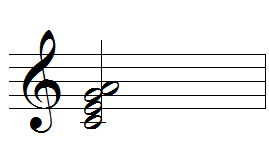
\includegraphics[width=1.6in]{diss_prospectus_cega.png}
\end{figure}

Up through section 20, Mehegan has labeled such chords (in the key of CM) as I$^{+6}$.  Beginning in section 21, we should be inclined to apply the label VI$^6_5$.  Even assuming a stable and unambiguous key center (here, CM), the literal notes of the chord no longer suffice to determine its proper label; the exact same chord in Figure 3 receives the label ``I+6" on p.\ 30, while it is parsed as ``Am$^6_5$" on p.\ 45 (corresponding to VI$^6_5$ in our hypothetically-unambiguous CM key).  Chord identity is now fundamentally fuzzy,\footnote{I mean ``fuzzy" in the mathematical, set-theoretic sense; some II chords may now seem ``more-II-like" than others.  This concept is fruitfully imported into the music theory literature by papers like Quinn 1997 and 2001.} as non-tertian pitch structures may be identified as root-position triads with added notes (in figured-bass terms) or as inverted triads with or without added notes (in fundamental-bass terms).

%Bring in discussion of function here?
In the case of Figure~\ref{am_bigu}, the labeling distinction seems to have little impact on a resulting theory of syntax.  In the western classical syntax assumed by Mehegan, both VI and I$^{+6}$ (to keep Mehegan's terms) have a kind of ``tonic function" in the music of Chopin and other romantic composers, if we partake of the functional harmonic tradition traceable back to Riemann.\footnote{Tonic, subdominant, and dominant functions are first systematically laid out in Riemann's \emph{Vereinfachte Harmonielehre oder die Lehre von der tonalen Funktionen der Akkorde} of 1893.}  In Riemann's usage, the two chords are similar in that they are closely related: one is the relative minor (or major) of the other.  This claim of similarity does not require an examination of the actual successive deployment of these chords (i.e., their behavior in chord progressions), but rather a process for reducing one to the other used to construct a kind of structural equivalence class.  To Riemann, this similarity gives rise to the fact that I and VI are used in similar progressions-- and it is to this shared pattern of use that scholars usually refer when they discuss ``functional" harmony.\footnote{See, for example, Tymoczko 2011 \S 6.4 (pp.\ 212-214) and Chapter 7 (pp.\ 226ff).}  

Mehegan seems to use an adjusted and more specific notion of function, claiming that ``I$^{+6}$ is also VI$^{6}_5$, but the function of the chord is usually an adjusted I chord rather than an inverted VI chord."\footnote{Mehegan 1959, p.\ 47.}  This ``tonic function" has no necessary connection to the labeling procedure he employs, and it is evidently tied to the behavior of the chords in harmonic progressions-- their syntax.  To borrow terms from the linguistics I will discuss below (in \S 4), users of Riemannian function and Mehegan's function both construct syntactic categories, ``phrase constituents" of sorts which characterize the categories' members by the well-formed progressions in which they are involved.  In saying that the function of an ``adjusted I chord" differs from that of ``an inverted VI chord," Mehegan seems to make a subtle distinction between two different musical parts of speech.  The rules of a harmonic syntax should teach us how to order the things we identify as phrase constituents; if those things are categories of chord function, then we need a lexical classification scheme (telling us which kinds of chord fall into each category) and a set of syntactic progression rules (telling us which progressions are well-formed).

In this case, the lexical categories into which the ambiguous chord could be placed are likely to behave similarly with regard to the rules of the syntax.  This means that our labeling decision has a relatively small impact on what kind of syntax we are likely to describe for a passage (or style) in which the chord of Figure~\ref{am_bigu} features.  And aside from function, we might expect to use the assumptions of centricity and chord construction to help break the label degeneracy.  If the key center is $CM$, chords built on scale degree $\hat{1}$ are probably (though not necessarily) more frequent than chords built on scale degree $\hat{6}$, and if the most common chord construction involves placing the root in the bass, we ought to be willing to label the chord I$^{+6}$.  This might get us out of trouble in comparatively simple cases.\footnote{Note that the problem multiplies as even diatonic cases become more ambiguous.  An analogous appeal to centricity and root-position chord construction might lead us to label $CM: (F,A,C,D)$ as IV$^{+6}$ instead of II$^{6}_5$, though this might suggest that we acknowledge a much wider application of IV \emph{vis-a-vis} II than is commonly accepted in the literature. And what about the chord $(E,G,A,C)$?  Even if we are certain that the key is CM, is this some kind of inverted I$^{+6}$ (for which our symbols would fail us-- perhaps I$^{+6,6}$ or I$^{6,+4}$), or a VI$^{4}_3$?  Or, less probably, if we take Mehegan's supposed figured bass very literally, is this some kind of III$^{\sharp 5, +4}$?}  Consider, however, the more difficult case given in Figure~\ref{phry}, where centricity and chord construction are unlikely to help us and the consequences of our labeling are significantly greater for our resulting syntactic description.
%FIGURE 4: SOME COMPLICATED NON-TERTIAN CHORD THAT MIGHT BE AN INVERTED CHORD
\begin{figure}
	\centering
	\caption{An ``E Phrygian" chord, used in Mark Levine's introduction to Sus and Phrygian chords.}
	\label{phry}
	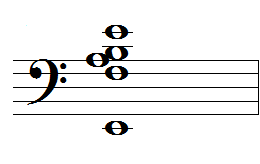
\includegraphics[width=1.6in]{diss_prospectus_ephryg.png}
\end{figure}
%Footnote it someplace: \footnote{Levine 1989, p.\ 25.}

In cases like these, the application of RNs can result in many different labels, depending on which assumptions and procedures we preference.  The chord does not immediately appear tertian in construction; no amount of inversion will allow us to rearrange this verticality as a stack of thirds.  The general reaction to non-obviously tertian or diatonic chords in jazz seems to consist in producing a story of its generation in which the ``unusual" sonority is neutralized by its reduction to more ``normal" chords, a sort of modern-day replication of Riemann's tendency to reduce chromatic chords to expected functions.  Mehegan's text does not provide one for the chord of Figure~\ref{phry}, which rose to prominence only in the 1960s, so we might turn to the later work of Mark Levine for help.

\subsection{Use vs.\ Pitch-class content}
Levine employs primarily lead sheet notation for his examples, eschewing RNs whenever possible.  To make sense of the chord in Figure~\ref{phry}, Levine starts by notating a ``G7" chord.\footnote{Levine 1989, p.\ 25.  It is worth noting that his G7 chord contains the registrally-ordered pitches (GFABE); the re-ordered stack of thirds would be (GB-FA-E), where I have placed hyphens in the place of omitted notes.  ``G7" thus stands as a rather incomplete (or at least classically atypical) description of the chord, which contains no fifth and an added ninth and thirteenth.}  Levine considers this to be a dominant seventh chord, thanks to its structural major third and minor seventh above the root.  Inverting the G7 to place the E in the bass, according to Levine, changes the function of the chord: ``Even though G7 is a V chord in the key of C, the V-I relationship here is between E and A."\footnote{Ibid.}  Here, we see one of Levine's rare appeals to RNs.  Evidently, while the \emph{configuration} of this chord (that is, the pitch and interval content) does not indicate its syntactic role as V in A (it is missing a third, fifth, and seventh), its \emph{function} is nevertheless a dominant one in this key, and Levine likens it to a classical ``Phrygian" cadence.\footnote{This dominant flavor might come from the $\flat$9 above the bass; Levine constructs dominant sevenths with this interval in chapter 8 (see p.\ 49).}  When Levine uses the term ``V," he establishes a lexical category quite different from the vertical structure-oriented categories seen in Mehegan's work: here, the pitch class set entirely matches that of a G7 (up to Levine's voicing options, not rehearsed here), but the ordering and deployment of the set instead places it into the category of a V chord in A-- despite its missing third and seventh, two notes considered important to a chord's functional identity.  We seem to be forced to label the chord either by its pitch content or by its use, and the resulting application of RNs is left ungrounded.  ``V" may no longer resemble a diatonic, tertian seventh chord, but rather a lexical category of morphologically dissimilar entities which function in similar ways.

In the context of a passage in AM, the choice of label for this chord provides ideas of syntax which differ more than in the case of Figure~\ref{am_bigu} above.  If we choose to label it as an inversion of G7, our syntactical parsing will reflect a RN motion $\flat$VII-I; if we choose E Phrygian, the ``root" motion between two chords will instead lead us to describe the harmonic progression as some kind of V-I motion.  The resulting theory of syntax will be guilty of question-begging; in assembling the labels off of which the syntactic observations will be based, we must invoke the contextual syntax itself to override or augment a pitch class set-based lexical classification scheme.

In order to explain away the pitch class content of chords like this when placing them in a structurally-unexpected lexical category (like one based on the V function), analysts employ a variety of reductive techniques designed to account for the disparity between a chord's contents and its contextual, use-based label.  Syntactic demonstrations drawing on methods like those of Mehegan and Levine would then trace the following path:
\begin{enumerate}
	\item Begin a description of jazz syntax by categorizing chord-to-chord successions.
	\item Establish figured bass-oriented labels based on centricity, diatonicity, and tertian chord construction (though the latter two of these assumptions can be relaxed); implicitly identify fundamental bass (via root tones) with figured bass (via bass tones).
	\item Notice that non-tertian and/or non-diatonic pitch stacks lead to fundamental bass ambiguity; figured bass and structural descriptions no longer capture intuitive sense of use (or lexical categories representing function).
	\item Abandon figured bass labeling in an attempt to indicate function; create generation/reduction procedures relating non-tertian/non-diatonic pitch stacks to centered, diatonic, tertian chords.
	\item Demonstrate syntactic function from the resulting labels-- though our assumptions about the expected nature of such syntax strongly informed our application of these labels in the first place.
\end{enumerate}

At stake here is not merely what notation we use to describe the E Phrygian chord.  Any syntax which purports to describe well-formed sequences of RN lexical categories based on centricity, diatonicity, and tertian construction will stumble with chords whose functional use seems to defy those structural categories, whether due to voicings, alterations, or some contextual phenomena.  It seems that the search for RN-based syntax requires syntactic assumptions for the generation of RNs.  If we wish to test a jazz repertory for syntactic progressions, we will need to first identify lexical categories in some more neutral way.

\section{Syntax in Music}% Syntax(es) and Musical ``Depth"}

In claiming identical ``rules and conventions" for jazz harmony and classical harmony, Mehegan's claim (1) subsumes several separate statements about conventional similarity.  First, it implies that the individual genres of Bach fugues, Mozart sonatas, and Brahms rhapsodies each have relatively homogeneous ``rules and conventions."  Second, it implies that these three sets of conventions are instantiations of an overarching set of rules called ``classical harmony;" while Brahms sounds like Brahms and Bach like Bach, there is some shared backdrop of harmonic processes at play in the works of classical composers.  Third, it implies that jazz music partakes of a homogeneous set of rules and conventions called ``jazz harmony."  Lastly, statement (1) above explicitly claims that the set of rules of this general jazz harmony are identical to the set of rules for general classical harmony.

I am deliberately (and somewhat unjustly) interpreting Mehegan's claim literally in order to indicate the complicated and potentially-contradictory conditions a harmonic theory must meet in jazz or any other music.  Mehegan does not pursue a monolithic and faceless jazz harmony; rather, in the remaining volumes of his work, he describes the practices of several prominent jazz pianists\footnote{In Vol.\ 3 consists entirely of individual studies devoted to Teddy Wilson, Art Tatum, Bud Powell, George Shearing, and Horace Silver, and Vol.\ 4 foregrounds the work of Oscar Peterson and Bill Evans.} in order to articulate a network of harmonic conventions, some of which are shared between many groups of performers (such as the A and B voicings of Vol.\ 4), and some of which are more typical of one practitioner or form of jazz practice than of others.\footnote{Some of the individualized tendencies Mehegan identifies relate to patterns of alteration.  For example, Mehegan claims that some of Bud Powell's ``persistent idioms" consist of deploying raised 4th and 7th degrees and both raised and lowered 2nds above the root over ``Dominant Chords" (Vol.\ 3, p.\ 120).  Mehegan thinks that the structure of a dominant seventh chord exists behind (in some conceptual sense) the chords deployed by Powell and others, but that the notes which appear in the actual voicing of the chord and the resulting melodic lines are more a matter of individual preference.}  Mehegan clearly thinks that a relatively coherent set of harmonic ``rules" regarding chord structure and succession sits in the shared background of these forms of practice, but he also seeks to articulate differing interpretations of these rules.  Just as ``common practice tonality" provides a set of guidelines within which Bach fugues, Mozart sonatas, and Brahms rhapsodies participate with different conventions and practices, a successful theory of jazz harmony must describe a shared set of jazz harmonic rules, if one exists, and also allow us to describe the practices of particular jazz ``communities," be they geographical, temporal, or abstractly metaphorical.

To borrow a concept taken from Richard Wollheim and developed Whitney Davis, I might describe Mehegan (and Coker, among others) as a type of \emph{latent formalist}.  Latent formalists seek to describe a form of artistic practice by appealing to a language-like system underlying the surface organization and configuration of works.  A latent formalist description of a work then appeals to a set of syntactic rules which make the surface intelligible.  Mehegan thinks that each jazz musician he seeks to describe has a distinctive harmonic style composed of elemental techniques rendering it sensible and recognizable, a ``rule-book" providing ``a general method of [musical] composition."\footnote{Davis 2011, p.\ 59; I have replaced Davis's term ``pictorial" with ``musical," which I do not think changes the spirit of his remarks.}  ``Latent Formalism," as Davis describes it, ``claims to reconstruct the system behind such methods, the recipes and rules."\footnote{Ibid.}  Like Davis's latent formalists, the task of many jazz theorists seems to be to replicate the methods of jazz pianists by providing syntactic rules distilled from observation of the works themselves.

What is the nature of these harmonic rules and conventions?  The history of writing about music is littered with both typological and contextual laws meant to indicate which sonorities are appropriate or pleasing and when they might be deployed.  In the typological genre, I count traditional dicta regarding consonance and dissonance\footnote{For a good overview of these kinds of claims from a jazz perspective, see McGowan 2008.  We might also call arguments over whether a sound is musical or not (say, a lawn mower) similar in structure.} and restrictions on what kind of verticality is or is not permitted in ``musical" utterances generally-- rules of the form ``tritones, bird song, and car horns are not permitted in civilized music, while major and minor triads are."  Mehegan makes a claim of this nature when he asserts that ``Chords of less than a seventh are insufficient for jazz."\footnote{Vol.\ 1, p.\ 11.}

On the contextual side, I refer to descriptions of permissible sequences of verticalities-- rules of the form ``vertical array X may [not] follow vertical array Y."  Appealing to the circle of fifths, Mehegan offers contextual rules like ``III normally moves to VI."\footnote{Vol.\ 1, p.\ 158.}  Whether based on supposedly natural laws, spiritual guidance, or examination of a specific repertoire, these ``laws" aim to articulate a set of constraints within which harmonies and their temporal orderings are recognized as appropriate and musical.  To phrase this in a more provocative way: these laws outline criteria for the well-formedness of harmonic successions.  They might be seen to form the basis for treating ``a work of art as if it had a linguistic identity or at least a language-like identity" -- the harmonic forms deployed by musicians are then ``constituted within the system in the same way as a well-formed sentence might be spoken by someone who knows the grammar of a language."\footnote{Davis 2011, p.\ 58.}  As a latent formalist like Mehegan considers the well-formedness of harmonic successions, he analogizes the process of constructing a solo to that of constructing a linguistic utterance.  I will return to critiques and framings of latent formalism in Chapter 5, while what follows here unpacks the linguistic ramifications of such approaches.

\subsection{Well-Formed Language and Linguistic Components}

To describe the search for harmonic rules as the establishment of criteria for well-formedness is to partake of a twentieth-century music theoretical tradition whereby terminology and methods are imported from linguistics (and through linguistics, mathematics and formal logic).  In music, as in so many other fields of the humanities, this means almost exclusively to borrow from the fertile and divisive ideas of Noam Chomsky.  Chomsky's \emph{Syntactic Structures} (1957) and \emph{Aspects of the Theory of Syntax} (1965) lay the groundwork for a structural and quasi-cognitive model explaining (or at least describing) the distinction between well-formed and malformed utterances in spoken or written language.  In these early works, Chomsky partitions linguistic performance into three interlocking components: the phonological, the semantic, and the syntactic, the last of which is of primary interest to him.\footnote{Chomsky 1965, p.\ 16.}  In language parallel to that of Mehegan, Chomsky defines syntax in passing:

``[This study] will be concerned with the syntactic component of a generative grammar, that is, with the rules that specify the well-formed strings of minimal syntactically functioning units (\emph{formatives}) and assign structural information of various kinds both to these strings and to strings that deviate from well-formedness in certain respects."\footnote{Ibid., p.\ 3.}

This ``definition" itself includes the term syntactic, so I might rephrase it in simpler language to remove some of the ambiguity: the syntactic component contains the rules that specify the well-formed ordering of whatever objects for which ordering carries structural importance.  For the syntax Chomsky describes, formatives are words composed of phonemes, and sentences constitute well-formed strings of these formatives.  The rules to which Chomsky refers and the ``structural information of various kinds" are not contained in the sentences of the language explicitly; rather, the grammar hypothesizes them and judges their accuracy and usefulness by its resulting ability to generate all and only well-formed strings.

As I see it, the structure of this syntax is informed by two key observations.  First, some English sentences can be grammatical without being sensible; the well-worn example is Chomsky's novel sentence ``Colorless green ideas sleep furiously."\footnote{Chomsky 1957, p.\ 15.}  For Chomsky, this sentence can be parsed syntactically with little problem; the subject is a noun phrase in which colorless and green are adjectives modifying ideas, and the adverb furiously modifies the action of ideas (sleep).  Semantically, however, this sentence fails to satisfy a literally-minded listener.\footnote{Though other scholars and artists have offered abstract or metaphorical interpretations of the sentence in an effort to render it ``sensible."}  This type of semantically-malformed sentence differs from syntactically-malformed sentences like ``Furiously sleep ideas green colorless"\footnote{Chomsky 1957, p.\ 15.} or ``sincerity frighten may boy the."\footnote{Chomsky 1965, p.\ 76.}  If sentences may be syntactically acceptable without being semantically parseable, the two linguistic components must be separable, at least to some degree.  Accounting for this phenomenon leads Chomsky to posit a deep syntactic background independent of and as input to semantic processing.

Chomsky's second guiding insight is the recognition that many apparently different sentences can be well-formed and convey the same semantic content.  That is, the differing ``surface structures" and phonological interpretations of sentences like ``I expected a specialist to examine John" and ``I expected John to be examined by a specialist" nevertheless correspond to identical deep structures upon which their semantic equivalence seems to be based.\footnote{Chomsky 1965, p.\ 22.}  Chomsky's syntax must now perform a difficult double duty: it must determine the phonetic interpretation (the sounding order and cadence of phonemes) as well as the semantic interpretation (some information regarding a referential claim to ``meaning") while preserving the possibility of similarity in one domain alongside difference in the other.  ``Consequently," he writes, ``the syntactic component of a grammar must specify, for each sentence, a \emph{deep structure} that determines its semantic interpretation and a \emph{surface structure} that determines its phonetic interpretation.  The first of these is interpreted by the semantic component; the second, by the phonological component."\footnote{Chomsky 1965, p.\ 16.}  Having isolated the syntactic component of linguistic ability, Chomsky partitions it into distinct levels, one of which must necessarily stand as an abstraction from the observed ``surface."

At this point, it might be productive to take a brief aside in the form of a series of caveats for those of us interested in applications of Chomsky to music theory.  First, Chomsky's model of linguistic components and their ordered interrelation sparked a fierce debate centered around the competing view of semantics as a generative ground for syntax, rather than as a recipient of syntactic structure as input.\footnote{For an eloquent exposition of this position, see Jackendoff 1990.  The resulting ``Linguistics Wars" are well-documented in Harris 1993.}  Second, it is not entirely clear to what degree jazz (or any music) functions as a language; does it have semantics distinct from syntax, for example?  And third, Chomsky continued to develop and modify his views over the next three decades, complicating or undermining some aspects of his early syntactic system.  While many of the structural specifics I will discuss below change between \emph{Syntactic Structures} and \emph{The Minimalist Program}-- sometimes, I will argue, in ways significant to music theory-- the general model of linguistic components outlined above emerges largely unscathed.  The nature of Chomsky's alterations involve primarily the syntactic component itself.  As incentive, I offer a provocation: the first importations of Chomsky's linguistic ideas into music theory happened in the works of authors like Winograd (1968) and Lerdahl and Jackendoff (1977 and 1983), well before the emergence of the ideas associated with Chomsky's Minimalist Program.  If Chomsky himself critiques some aspects of his early thoughts on syntactic structure, then perhaps we, too, could benefit from turning a critical eye on the linguistic machinery we borrow to make sure it isn't out of date.  The parts that wear out over time may help us to identify breaking points in music theory-- and perhaps in the analogy between music and language in general.

\subsection{The Syntactic Component: How Deep?}
In order to account for the two observations I highlight above, Chomsky's syntactic component (as interpreted in Chomsky 1957 and 1965) must support two representational levels-- a ``surface" level fed to the phonological component and a ``deep" level given as input to the semantic processing faculties.  Under the influence of symbolic representations of mathematical logic, Chomsky seeks to account for well-formed strings by showing that they can be generated by a small number of ``rewriting rules" which replace one symbol with another; on a deep level, rewriting rules allow for the elaboration of one phrase constituent into others, and on a surface level, rewriting rules allow for the modification of one or more phonemes/morphemes.\footnote{Chomsky's argument for the conceptual primacy of these rewriting rules seems to be a combination of an appeal to intuition plus a demonstration of effective results.  See, for example, Chomsky 1965: ``It seems clear that certain kinds of grammatical information are presented \emph{in the most natural way} by a system of rewriting rules, and we may therefore conclude that rewriting rules constitute part of the base of the syntactic component" (p.\ 67; emphasis mine).}  Repeated application of rewriting rules from an initial symbol for ``sentence" yields the iconic syntactic derivation trees prominent in Chomskyan linguistics.  Chomsky's sentence derivations proceed from the top down in that the initial sentence symbol is rewritten into symbols like ``NP and VP," each of which can be rewritten by other rules into phrase structures of essentially arbitrary complexity.

This arbitrary complexity worries Chomsky, to some extent, who thinks that any grammatical theory should, on some level, significantly simplify the plethora of phrases accessible to and generatable by the grammar.  In order to winnow down the number of rewriting rules and phrase structures to what he considers to be a cognitively-plausible core, Chomsky separates the phrase constituent rewriting rules of the deep structure from what he terms to be ``grammatical transformations," which produce the surface structure.  All simple sentences, he claims, can be generated by the essential rewriting rules of the deep syntactic ``base"-- loosely, these sentences form the kernel of the language.\footnote{Chomsky later nuances this, claiming that some transformational rules (that is, rules outside the base rewriting rules, proper) are ``obligatory," while others are ``optional"; the revised kernel, then, consists of sentences to which the obligatory transformations have been applied (cf. Chomsky 1965).}  The strings generated by the rewriting rules of the deep syntactic structure determine the semantic interpretation; these strings need not, however, appear directly on the (phonological) surface, since subsequent transformations may change numerous properties of the string ranging from word ordering to activity/passivity to tense constructions.\footnote{``Thus the syntactic component consists of a base that generates deep structures and a transformational part that maps them into surface structures.  The deep structure of a sentence is submitted to the semantic component for semantic interpretation, and its surface structure enters the phonological component and undergoes phonetic interpretation" (Chomsky 1965, 135).}  To tie this configuration to the two guiding observations I noted above: the possible syntactic nature of non-semantic utterances can be derived from the proper arrangement of phrase constituents arising from the syntactic base (but improperly submitted to the semantic component), and the semantic correspondence of differing phonetic structures is accounted for by their shared deep structure (but different application of transformation rules in the generation of their surface structures).  If Chomsky can reduce many \emph{a priori} different sentences to a small number of deep structures and a collection of shared transformational rules, he can demonstrate an attractive simplicity to his grammatical theory and a comparatively low cognitive demand.

Chomsky contrasts this approach with what he views as the position of modern structural linguistics, claiming that ``one might briefly characterize the syntactic theories that have arisen in modern structural (taxonomic) linguistics as based on the assumption that deep and surface structures are actually the same... The central idea of transformational grammar is that they are, in general, distinct and that the surface structure is determined by repeated application of certain formal operations called ``grammatical transformations" to objects of a more elementary sort."\footnote{Chomsky 1965, 16-17.}  Chomsky polemicizes against this ``taxonomic" linguistics; to him, any structural system which does not reduce many differing sentences to a small(er) number of deep structures must become complex and unwieldy, at best, and inaccurate, at worst.  The different ``branching off points" of Chomsky's semantics and phonetics, so to speak, can be accommodated in a syntactic system with a single structural level only clumsily.  Treating the surface as the structure of grammatical importance leads to a system that is both semantically and cognitively dubious.

\subsection{Structural Levels and Music}
%This appealed to theorists
The linguistic description of this multi-level, generative apparatus, where the ``deepest" level of structure is an abstraction from the surface but is thought to give rise to the surface in some way, seems to have come as both an exciting development to computer scientists with interests in language/music processing and as a relief to music theorists familiar with western tonal harmony-- especially to those who aligned themselves with the tools of Heinrich Schenker.  Early Schenkerians ranging from Salzer and Schacter to Forte long postulated distinct harmonic structural levels as the basis for their descriptions and explanations of tonal compositions.\footnote{For representative examples, see Salzer and Schachter 1989, Forte 1959, and Forte and Gilbert 1982.}   At the same time that Chomsky's early syntactic work began to revolutionize linguistics, Forte praised Schenker's ``achievement-- which might be termed the deepening of musical understanding through the discovery of the principle of structural levels."\footnote{Forte 1959, p.\ 4.}  As Forte reads it, a Schenker graph consists of a tripartite structure, where ``the lowest staff contains the major surface events... Schenker has designated this level as the \emph{foreground}," while ``on the upper staff, he has represented the fundamental structural level, or \emph{background}, which controls the entire work."\footnote{Ibid., p.\ 8 (emphasis Forte's).}  Despite complicating factors introduced by the middleground, consisting of ``structural events which lie immediately beyond the foreground level,"\footnote{Ibid., p.\ 8.} in some intermediate space between the governing background and the perceptual foreground, the direct similarity to Chomskyan syntax seems clear: the sounded surface structure is somehow generated from an abstracted background, which may itself underpin several seemingly-distinct utterances (be they sentences or pieces).

The planting of Chomskyan seeds in this structurally-fertile soil resulted in an overlapping array of approaches:\footnote{For a helpful overview of early approaches to Chomsky-influenced musical grammars, see Roads and Wieneke 1979.}  where generative syntax met Schenker, scholars pursued projects attempting to formalize harmonic structural levels in music;\footnote{The touchstone for this approach is the work of Lerdahl and Jackendoff, discussed below.} where generative syntax met the influence of symbolic representations and computational methods, scholars applied Chomskyan generative tools in the absence of explicitly Schenkerian methods and tailored them toward the use of computers in the analysis and production of music.\footnote{Explicitly generative but not necessarily Schenkerian projects of this style include Winograd 1968, Laske 1972 and 1975, and Steedman 1984; this thread may be later traced through Keller and Morrison 2007 and Rohrmeier 2011.}  After discussing each of these in turn, I will highlight the work of theorists who employ some concepts of grammatical syntax in a computational setting without the explicit importation of Chomskyan generative structural levels; it is into this last camp which my project aims to fall.\footnote{See \S 4, where I will discuss statistical approaches which lack aspects of multi-level generative structure.}

Lerdahl and Jackendoff 1977 confronts the dual lineage of Schenker and Chomsky directly.\footnote{This early work is modified and included in the greatly expanded \emph{Generative Theory of Tonal Music} of 1983, but the methodological positioning \emph{vis a vis} linguistics remains unchanged.}  Lerdahl and Jackendoff's project is motivated by the observation that much previous (tonal) music theoretical work lacks systemic formalization.  ``Even Schenker's theory," they note, ``which can be construed as having much in common with the generative approach to linguistics, is at bottom inexplicit."\footnote{Lerdahl and Jackendoff 1977, p.\ 112.}  To emulate the success of Schenker's ideas while rendering his analytic method more explicit, Lerdahl and Jackendoff's stated methodology is ``patterned after the methodology of linguistics in that we demand strong motivation, formal rigor, and predictive power for every part of the theory," though they claim that they ``do not approach music with any preconceptions that the substance of [their] theory will look at all like linguistic theory."\footnote{Ibid.}  While the actual content of their systemic observations will be new, the authors follow a Chomskyan program of study in attempting to produce a set of formal rules (a grammar) which generate (in the predictive, rather than literal sense\footnote{Lerdahl and Jackendoff are careful to distinguish ``generate" in the mathematical sense from its more colloquial use, reminding readers that a generative theory of music need not produce any actual music.  Their goals are to produce a \emph{strongly generative} system, which provides structural descriptions to every musical utterance, rather than a \emph{weakly generative} system, which could generate a set of phrases but not necessarily their structural description.}) competent musical utterances.

The resulting generative rules are partitioned into several categories, much like the elements of Chomsky's grammatical apparatus:  ``the rules which assign structural descriptions are categorized as \emph{well-formedness rules}, which assign possible structures, and \emph{preference rules}, which select coherent structures from possible structures.  In addition, \emph{transformational rules}, which convert structures into other structures, are needed for special cases (such as elisions) not generated by the well-formedness rules."\footnote{Lerdahl and Jackendoff 1977, p.\ 116.}  For a given musical utterance, the well-formedness rules generate an array of possible structural descriptions which resemble parsing trees.  These trees attempt to abstract from the surface down to a description of the most important events by removing one level of surface elaboration at a time.  Not all of the resulting trees allowed by the well-formedness rules will appeal to the intuitions of an educated listener equally, however; the preference rules are meant to differentiate between structural descriptions along a scale of plausibility.  This differs somewhat from early-Chomskyan generative linguistics, where a sliding scale of grammaticality plays no explicit role.\footnote{See, for example, the claims of innovation and justification for preference rules in Lerdahl and Jackendoff 1985, especially pp.\ 154-157.}

Jackendoff, a prominent linguist and student of Chomsky's, is certainly no stranger to generative linguistics, and his importation of generative terminology and concepts like well-formedness, transformational rules, and parsing trees comes with a series of cautionary tales meant to intercept misreadings of generative terms and structures.  In particular, Lerdahl and Jackendoff warn against the facile identification of the Schenkerian background with Chomskyan deep structure, writing that ``neither the underlying levels in our reductions nor Schenkerian ``background" levels are deep structures in any sense analogous to deep structures in linguistics.  Rather, they are analogous to stages of phrase-structure analysis as represented in linguistic trees."\footnote{Lerdahl and Jackendoff 1977, p.\ 163.}  But Lerdahl and Jackendoff read the trees themselves as reflecting a relational/inclusional difference, ``since musical trees represent elaborations rather than ``is-a" relations among grammatical categories."\footnote{Lerdahl and Jackendoff 1977, p.\ 163.}  As they see it, the branching of the top level of a linguistic phrase-structure tree reflects that sentence S ``is a" NP plus a VP; this differs from a Schenker-style reduction, in which lower levels on the tree represent ``elaborations" of higher levels, which themselves are sounding entities, rather than categories.  ``Our musical trees," they write, ``do not involve grammatical categories.  The fundamental relationship which they express is that of a sequence of pitch events as being an \emph{elaboration of} a single pitch event.  The \emph{dominating} event, that of which a sequence of events is an elaboration, is always one of the events in the sequence; the remaining, \emph{subordinate} events in the sequence are heard as relatively ornamental.  ``Reduction" -- the process of recursively substituting single events for sequences of events -- can be thought of as the inverse of elaboration."\footnote{Lerdahl and Jackendoff 1977, p.\ 129.}

When confronted with a musical surface requiring harmonic parsing, then, Lerdahl and Jackendoff reduce away elaborating harmonies one at a time, moving up the tree and revealing ``dominating" events (note: not categories like NP and VP\footnote{The repeated assertion that placing a harmonic label like ``I" high up in a generative structural tree is not a categorical claim should perhaps be taken with a grain of salt; Lerdahl and Jackendoff see this move as elevating a literal and aural ``I" to a place of higher prominence, while I might instead argue that this merely establishes and labels a category of surface structures beneath it on the tree which can elaborate ``I."}) which bear syntactic relations to one another determined by the deep-structural principles embodied in the well-formedness rules.  The principles of underlying harmonic syntax, however, are not demonstrated, but assumed; one of the important areas left ``open" in the most complete statement of their project, \emph{A Generative Theory of Tonal Music}, is ``the wholesale assumption of traditional principles of harmony and voice leading."\footnote{Lerdahl and Jackendoff 1985, p.\ 154.}  It is these syntactic assumptions, alongside the authors' multi-faceted treatment of time spans and rhythmic parameters, which will directly inform the choice of dominating events during reduction.  If we wish to study harmonic syntax, the musical challenge to which a system built along these lines must rise centers precisely on the notion of reduction.  If (1) it were somehow obvious that the most important rules of harmonic convention were quite different from how they appear on musical surfaces and (2) there were a systematic and relatively assumption-free way to tell which surface features are dominating (in the above sense), perhaps we could provide a systematic account of harmonic structure which connects the well-formedness rules to the musical surface.

In other words, it seems that a \emph{prima facie} generative approach to music which borrows Chomskyan methodology (like a deep structure consisting of well-formedness rules) and inherits Schenkerian structural levels and reduction techniques cannot help us to understand syntax from first principles; rather, the process of reduction itself depends, to some extent, on the application of pre-existing notions of syntax.  In attempting to build a system of well-formedness rules and test them on well-known musical examples, Lerdahl and Jackendoff cannot simultaneously test the assumed rules of harmonic syntax themselves.  If the program produces an unusual or intuitively undesirable structural parsing, the authors adjust the well-formedness rules, preference rules, and transformations appropriately rather than consider changes to the paradigms of harmonic succession which inform their decisions.  While this is not undesirable for a theory of structural levels, it is undesirable for an investigation into the nature of syntax, and the issue comes down to the criteria of evaluation for the system's efficacy: the way to test a generative system like that laid out in \emph{GTTM} is to ``run" it on a corpus of musical examples and check how well the results match the intuitions of trained analysts.  But if the system's output structural analyses match well, that only means that it is possible to built a set of reduction rules which fit the surface data (that is, the pieces) to a hypothesized set of harmonic conventions.\footnote{Moreover, as I will claim in Chapter 5, ``running" an algorithmic parsing routine on inputs typically interpreted by human brains produces outputs which resemble or mimic human ones but which are involved in a different chain of reference and proof.}  In particular, it says nothing about whether there might be other sets of harmonic conventions that, when coupled with a differing generative system, might provide equal or better analyses.  In the classical case, where the general conventions of harmonic succession are widely accepted, this is no large road block, but in cases like jazz, the results could be unnecessarily reductive: even if a system of generative rules can fit the surfaces of jazz performances to the harmonic conventions of western classical tonality, the necessity of those harmonic conventions instead of other ones cannot be established.  Just because the harmonic motion of jazz can be made to resemble that of the tonal common practice does not mean that the same descriptive machinery must operate under the hood.  

I tend to doubt the importance of deep-structural generative approaches to harmony, especially those which require high degrees of recursion.  My project below, however, remains partly agnostic on this question.  On first glance, my work aims to describe harmonic syntax in jazz by appealing only to the surface in a quasi-Markovian way (to be discussed below); a dedicated generative theorist might, however, choose to read my work as a more direct investigation into what kinds of syntactic objects and successions we might permit in the harmonic conventions underpinning a set of Lerdahl and Jackendoff-esque well-formedness rules.  If the harmonic surfaces of jazz performances support different categorizations, generative theorists could then choose to pursue new (and hopefully simpler) sets of transformational and preference rules, building a generative system on structures different from the roman numerals of western classical tonality.  In keeping with the Chomskyan tradition, we might compare the fit by testing the fit of each rule system to musical surfaces.

But even testing the fit of any single generative rule system to the data, apart from the potential multiplicity of deep-structural harmonic conventions, requires considerable effort.  The formalized nature of generative methods, however, are of great assistance here: computer scientists quickly discovered that many types of generative rules could be encoded into symbolic programming languages efficiently and precisely.  Chomsky's treatment of language as a formal system might thus be said to bear unexpected fruit in bringing together the quasi-Schenkerian music analysis field of inquiry with computational corpus analysis under the shared banner of generative structure.

\subsection{Computational grammars} %Generative Grammar, Computational Methods, and Music
%There are non-computational generative people in music (like L&J) as well as computational ones (like Winograd and Rohrmeier?).  Leave a real description of my corpus analysis for later?
As Lerdahl and Jackendoff assembled their (largely classical) \emph{GTTM}, researchers interested in musical applications of computer science and machine and artificial intelligence seized on many of the same Chomskyan ideas, applying their symbolic representations to both ``classical" and jazz repertoires.  Starting with the works of Winograd (1968) and Laske (1972, 1973), computational explorations of grammars seize on two characteristics of generative structures: the symbolic specificity of well-formedness rules and the hierarchical embeddings of parsing trees.  Winograd starts by assuming ``the principles explained in Forte's Tonal Harmony in Concept and Practice, simplified as necessary to meet the goal of writing an effective grammar and parsing program."\footnote{Winograd 1968, p.\ 5.}  Directly and thoroughly invoking Chomsky, he then employs systemic grammar to fit musical pieces to agreeable harmonic structural parsings.  Numerically encoding musical notes, Winograd postulates well-formedness rules meant to generate the musical surface, complete with ``realization rules" similar to Chomsky's transformational rules.\footnote{Winograd 1968, p.\ 10.}  His computer deploys the realization rules in an attempt to produce ``a single `best' parsing (i.e. most in accord with the logic of tonal harmony)."\footnote{Winograd 1968, p.\ 30.  Winograd considers the selection of the ``best" parsing a semantic problem, and he ties it directly to harmonic function.  Observing that one chord can have many different functions in different tonal contexts, he identifies semantics as something separate from chord structure, formally speaking.  In this way, he seems to entangle syntax and semantics to a more significant extent than Chomsky's work does: Winograd's output parsings are meant to include function, so his ``syntactic" parser must really also rely on or include ``semantics," by his definitions.  I am unsure whether harmonic function is analogous to a semantic concern rather than a strictly syntactic one, but carrying the syntax/semantics distinction over into music in this way seems to cause more problems than it solves.  In particular, if function is a semantic notion, then what is left for syntax to specify?}  His system shares with Lerdahl and Jackendoff the goal of strongly generating harmonic structural parsings, and his computational methods are, in principle, generalizable to a large corpus.  They will not, however, aid in our investigation of ``the logic of tonal harmony," since they refer to Forte's assumed tonal logic both while producing all possible parsings and while selecting the ``best" one.

Encouraged by Winograd's computational ability to parse complex surfaces into deep syntactic structures and realization rules, Mark Steedman pursues similar goals in a jazz context in both linguistic terms (1984, 1996) and in directly computational ones.\footnote{See Granroth-Wilding and Steedman 2012.}  In his earlier work, Steedman generates harmonic parsings by hand for what he identifies as the most commonly deployed forms of the 12-bar blues, postulating a shared harmonic background (roughly I-IV-I-V-I) and constructing a set of transformational rewriting rules to account for many surface variants.  Each chord in the deep structural progression may take part in a series of branching and substitution procedures, producing language-like hierarchic embeddings. The same hierarchical structure makes its way into Steedman 1996 and Granroth-Wilding and Steedman 2012, but with updated linguistics, imported probabilistic computational methods, and a more ambitious goal-- that of producing an automated harmonic analysis routine.

In the latter of these, Forte's harmonic system is replaced with a \emph{tonnetz}-like system inspired by just intonation and indexing chords only by their root.\footnote{See Granroth-Wilding and Steedman 2012 \S 3, ``A Model of Tonality."}  Localized motions in the resulting tonal space stand as well-formed deep structures.  Drawing on methods established in Steedman 1996, the authors then construct the lexicon for a combinatory categorial grammar (CCG), a grammar where utterances are assembled out of item-to-item structural constraints contained in the choice of lexical category.\footnote{As an example, a chord parsed into the category ``Dom" would be deployed directly before a chord from the ``Ton" category, where both categories are defined by the relationships between the roots of the chords placed in them.}  A CCG partially defines its categories by the combinations in which category members participate.  This functional orientation is similar to that employed by Levine and other theorists when grouping chords by behavior, rather than by configuration.

Steedman and Granroth-Wilding, however, choose the categories of their CCG in advance, anticipating the kind of syntactic model they expect to use.  They then annotate jazz scores by hand, providing ``gold standard" parsings in terms of their CCG categories.  The statistics generated from this process (like how often category A progresses to category B or C) train the CCG how to produce the most probable node expansions-- that is, the most probable re-writing rules which expand one lexical item from the CCG into multiple such items.  This probabilistically-trained CCG engine is turned loose on jazz standards and allowed to generate its best guess for harmonic structural parsings.  If Granroth-Wilding and Steedman choose their CCG lexical categories in advance and annotate their musical data in terms of these categories, they still must make labeling decisions of the kind interrogated in \S 3 above.  The nature of the lexical categories will inform the resulting syntactic parsings.  Since the authors aim to demonstrate analytical parsings from an assumed underlying syntax, this method is effective.  But the syntax is still fit to the surfaces, rather than extracted from them.

More recently, the work of Martin Rohrmeier has continued the tonal generative investigations of Steedman and Lerdahl and Jackendoff.\footnote{See Rohrmeier 2007 and 2011 for a non-computational generative theory and Rorhmeier et al.\ 2013 for a description of hierarchical, generative musical grammar in the context of implicit learning.}  Rohrmeier argues that hierarchical tree structures capture and display tonal harmonic parsings uniquely well, and that the complexity of harmonic phrases exceeds our ability to parse them based only on chord-to-chord successions observable on the musical surface.\footnote{``...[T]he complexity of the underlying principles of structure building... exceeds Markov or finite-state models... Furthermore, linguistic as well as musical syntax is governed by tree structures and underlying recursive structures or grammars as part of their principles of structure building" (Rohrmeier et al.\ 2013, p.\ 3).  Rohrmeier makes similar claims elsewhere.  While Chomsky spends a great deal of time showing the inadequacy of Markov and finite-state models in the context of English, it is unclear to me that Rohrmeier 2007, Lerdahl and Jackendoff 1983, and Steedman 1984 establish this inadequacy in the case of musical harmony.}  While some of Rohrmeier's work explores the possibility of non-generative harmonic parsings,\footnote{See, for example, Rohrmeier's computational exploration of Markov models and Dynamic Bayesian Networks in Rohrmeier and Graepel 2012.} the majority of it accepts the framework taken from Chomsky and put forth by Lerdahl and Jackendoff and Steedman.

My skepticism of this framework is based on a couple of questions.  First, Chomsky introduced the separation of deep structure from surface structure to account for the shared semantics of dissimilar surfaces.  In music, I fail to see an equivalent motivation.  There may be cases where we might benefit from describing some shared quasi-semantic identity between two different harmonic progressions, but it does not seem to me that musical phrases have parseable meanings and referents in which to ground such semantic judgments.  Musical configurations might be thought to convey only syntactic configuratedness, rather than separately syntactic and semantic configuratedness.  In analogy with Chomsky's ``Colorless green ideas sleep furiously," can we construct harmonic progressions which make syntactic sense but violate some set of semantic considerations?

Second, Dmitri Tymoczko has called into question the plausibility and relevance of hierarchical recursion in tonal harmony.\footnote{See Tymoczko 2010.}  He notes that the hierarchical tree structures required by parsings like Rohrmeier's greatly exceed accepted linguistic trees in terms of recursive complexity, and that this sophistication is necessitated by our inability to parse harmonic progressions without them.  Echoing Chomsky, Tymoczko notes that ``In natural languages, it is impossible to recover the meaning of a sentence without recursive parsing;" the case of music, however, differs, since Tymoczko's results ``suggest that music can be comprehended according to local nonrecursive theory."\footnote{Tymoczko 2010, p.\ 4.}  Taking aim at Lerdahl and Jackendoff, Tymoczko claims that they ``provide few arguments, and little evidence, either against the traditional approach or for their recursive alternative; instead, recursive organization is explicitly assigned the status of a fundamental hypothesis."\footnote{Tymoczko 2010, Supplementary Materials, p.\ 9.}

If the appeal to recursive generative grammar is unmotivated by either arguments against local harmonic grammar or appeals to Chomskyan syntax/semantics separation, it seems more productive to me to consider surface temporal approaches to chord-to-chord succession.  The most promising candidate for a computational mechanism oriented in this direction may be the sort of Markovian approach advocated by Tymoczko 2010, though this work relies on RN labeling to make its claims.  Ian Quinn makes similar local harmonic grammar claims in the context of syntax-free labeling, and it is in this context that I wish to place my project.\footnote{See Quinn 2010 and Quinn and Mavromatis 2011.}

Quinn 2010 makes use of figured-bass labels which describe each chord as a set of pitch classes above the bass and relates adjacent sonorities to one another by comparing the interval between their respective bass notes.  Each verticality can be given such a representation without reducing away any of its notes on the basis of syntactic preconceptions.  Quinn tallies up every progression between these verticalities, clustering the results to look for patterns of harmonic behavior.  The resulting lexical categories assemble themselves on the basis of the chords' behavior-- they are not pre-defined, as in Granroth-Wilding and Steedman 2012 or Coker 1964.  The progression statistics generated in this way display the syntactic behavior of the corpus in question, rather than showing that the corpus can be fit to an assumed syntactic background.  This local grammar steers clear of my objections to generative grammatical investigations of syntax and frees its labeling from syntactic intuitions, though its success hinges on the highly-homogeneous texture and limited lexicon of the Bach chorales.\footnote{See Quinn 2010, \S 1.1, where the author explains that ``[t]he nature of the four-part chorale virtually guarantees that exactly four notes are sounding at any given moment...Clearly it is this property of chorales that gives us the latitude to define chord in a manner that is at once so broad and so black-and-white. We will set aside for now the question of the extent to which this definition can be carried over to other genres and other (non-MIDI) encodings."}  To pursue a minimally-reductive representation of harmonic progressions relevant to a jazz piano corpus presents more significant challenges, as Chapter 2 will outline.

\section{The YJaMP Corpus}
%Give an overview of the corpus

I assembled the Yale Jazz MIDI Piano corpus (YJaMP) between 2012 and 2014.  With financial support from the Yale Department of Music and the Allen Forte Fund, I recruited three highly skilled local jazz pianists to record on a realistic MIDI ``baby" grand piano located in the Department of Computer Science's ``Euterpea" studio.\footnote{This arrangement would not have been possible without the support of Ian Quinn, James Hepokoski, Sue Penney, Paul Hudak, and Donya Quick.}  The piano has the size, feel, and sound of a typical, acoustic baby grand -- but there are no strings, the soundboard has woofers in it, and the keyboard provides a MIDI line out with approximately 5ms accuracy.  While playing a MIDI piano in an isolated academic studio certainly does not mimic real performance conditions, this equipment provided the best experimental conditions available.  Each pianist commented on the realism of the piano's sound and action.

The pianists, Alexander Dubovoy, Julian Reid, and Joseph McWilliams, span different generations, educational histories, and career timelines.  Dubovoy and Reid, recent Yale graduates affiliated with the Yale Undergraduate Jazz Collective,\footnote{For more information on the collective and its schedule, see their Yale web presence at \href{http://campuspress.yale.edu/jazzcollective/}{campuspress.yale.edu/jazzcollective}} have studied with contemporary pianists like Craig Hartley.\footnote{Hartley's albums, marketing work, and scoring for site-specific art installations have begun to attract significant attention in New York and abroad.  For details, see \href{http://www.craighartley.me/}{http://www.craighartley.me/}}  McWilliams, an established pianist in the area, studied with earlier teachers -- including John Mehegan.

Each pianist recorded solo performances for one or two hours per session spread out over several months.  In an attempt to influence the style of the performers as little as possible, I made only two guiding requests: (1) that they should play ``Real Book-type tunes," a category I left deliberately vague, and (2) that they should play however they would typically play at a solo gig.  The first request encouraged the performers to play ``standards" material; the vast majority of the tunes they chose to play (and identified for me by their preferred title) can be found in one of the Real Book's published volumes.\footnote{For the ``official" Hal Leonard Real Book publications, which are themselves something of an oxymoron, see \href{https://officialrealbook.com/}{https://officialrealbook.com/}.}  Since the long jazz tradition of circulating ``real" and ``fake" books of tune lead sheets has a complex history, I avoided restricting the performers to any particular book.\footnote{I thank Brian Kane for sharing his insightful explication of the ontological ramifications of this network of replications (forthcoming).  See also the extremely informative Kernfeld 2006.}  In a handful of cases, pianists played tunes they considered standard-worthy but unrecognized, including ``covers" of original compositions by Radiohead and Robert Glasper.

As a result, the YJaMP corpus includes 189 distinct performances of tunes, constituting approximately 50,000 ``chords."  I employ quotation marks here to signal that I define ``chord" in a particular way suited to computational techniques, as seen in Chapter 2.  To preserve as much of the temporal structure of the MIDI performances as possible, these tunes are never quantized into traditional score notation, and the question of what defines the boundaries of a chord is non-trivial.  For now, I note that the estimate of 50,000 is higher than traditional score notation would suggest and lower than the number produced purely by ``salami slice" methods of White and Quinn.\footnote{See Chapter 2 and White and Quinn 2016.}

I do not mean for a corpus representing the work of three pianists to stand in for all of jazz, or even for all solo jazz piano in this time frame around the New Haven metropolitan area.  Rather, it provides a unique grounding combination of consistency (in that each pianist employs some voicings, progressions, and techniques common across many of their performances) coupled with noisy variety (in that each pianist interprets standards differently and employs different kinds of chords from the others).  Future work could attempt to isolate the precise statistical differences between each pianist's captured style, but my work here merely seeks to show that even a small community of partly-related practitioners can provide sufficient context for establishing temporal syntactic norms of harmonic behavior.  The methods are generalizable to other, similarly-represented corpora, both within the jazz community and outside it.  I hope what follows serves to direct our attention both to the commonalities between this corpus and broader expectations and claims regarding jazz harmony and to the ways in which the idiosyncracies of the corpus may suggest their own, non-totalizing descriptions.

\section{Toward a Corpus-driven Jazz Syntax}
%TODO: align the below with a stripped-down outline of my dissertation.

With a rich corpus in hand, I am inspired by Tymoczko, Mehegan, and Quinn to pursue a locally non-recursive computational syntax (Tymoczko 2010) willing to modify or dispense with traditional jazz chord labeling (Mehegan 1959) in favor of a data representation amenable to elementary machine learning techniques like unsupervised clustering (Quinn 2010).  I add to these fertile ideas a commitment to embed statistical temporality at each stage of the resulting analytical pipeline and a desire to frame carefully its computational and human interpretations and extensions in semiotic terms.

%ch 2
Chapter 2 approaches two different kinds of non-RN chord labeling techniques accountable to the YJaMP data: voicings and local scale-degree sets.  Both allow the analyst to capture a wide variety of chord constructions, tertian or otherwise.  Shedding the assumption of tertian construction renders the labeling system flexible enough to describe dense, chromatic clusters, quartal stacks, and ``extended" chords.  While theorists like Levine start by describing chords as stacks of thirds, they often advocate the deletion of one or more chord tones (especially the chordal fifth) so frequently as to suggest a general rule: ``tertian" chords are stacks of thirds, except the fifth is unnecessary.  But if chords like $(GBF)$ turn out to be more common than chords like $(GBDF)$, is it helpful to describe the former as an incomplete or modified form of the latter?  ``Tertian" chords linked by tone-removal and cardinality change often do participate in similar syntactic progressions, but the chord labeling system I employ will demonstrate this-- not assume it.

Of the two labeling systems Chapter 2 introduces, voicings (especially as indexed by salami slices) produce a large, sparsely populated lexicon ill-suited to machine learning generalizations, while scale-degree sets (especially as produced by optimizing pitch-class temporal distribution parameters) retain agnosticism regarding acceptable chord structures while reducing the lexical size.  I frame the production of chord objects from the surface data of the corpus with semiotic concepts drawn from the work of Paul Kockelman.\footnote{As later chapters will indicate, I find the model produced in Kockelman's \emph{Agent, Person, Subject, Self} (2012) and employed in papers like ``The Anthropology of an Equation: Sieving Spam, Algorithmic Agents, and Ontologies in Transformation" (2013) uniquely clear and flexible enough to capture much of how I interpret the acts of computational classification and analysis.}  Attending to the semiotic processes permitting communication between algorithmic and analytical agents both blocks misinterpretation of computational outputs and allows the alignment of object selection with the harmonic clustering concerns dependent on it.

%ch 3
Chapter 3 uses the ``$ii$" chord as a case study to situate scale-degree set chord progressions firmly in time.  Rather than defining chord progressions as notional bigram adjacencies and producing a complex set of rules designed to reduce musical surfaces to such adjacencies, I generalize ``progressions" at several data-driven time scales.  Python-based computational methods allow me to represent each scale-degree set in terms of the other chords to which it tends to progress, both immediately and after time delays of up to 5 seconds.  Dimensional reduction algorithmic work suggests three prominent ``temporal progression regimes," which I connect to intuitions regarding short-range voice-leading processes, syntactic transitions, and long-range, key-oriented harmonic norms.  In analogy to linguistics, I suggest labels legible to algorithmic agents based on the behavior of chords across phonetic, syntactic, and background regimes.

%ch 4
Chapter 4 deploys the temporal progression regime representation introduced in Chapter 3 across all of the most frequently appearing scale-degree sets in the YJaMP corpus.  After introducing a simple metric assessing the distance between any two scale-degree sets, I show that agglomerative clustering produces groupings of scale-degree sets resembling traditional expectations for syntax-preserving chord substitutions.  Unsupervised clustering and supervised classification provide the means for placing any scale-degree set into a bottom-up categorical structure.  The resulting syntactic groupings depend exclusively on statistics drawn from the temporal deployment of chords -- not on their pitch contents.

%ch 5
The pipeline of Chapters 2-4 produces syntactic categories free of some types of analytical circularity, but the latent formalist implications embedded in the pipeline are better suited to some modes of inquiry than others.  Chapter 5 returns to the jazz analytical literature to frame formalist harmonic analysis in terms drawn from both Kockelman and historian of art Richard Wollheim.  I describe my project not as a proof or disproof of any particular harmonic theory, but rather as a new paradigm under which some harmonic progression claims might be produced in an accountable and useful way.  I cast harmonic syntax, conceptually, as the result of a dense interconnection between content-driven and context-driven semiotic processes, and I indicate future projects designed to play to the strengths of a corpus-driven algorithmic pipeline.  Ultimately, jazz syntax stands here for harmonic syntax generally: an emergent set of properties dependent on the particular alignment between performance data, chord representation, and statistical patterns of temporal deployment.
